% !TEX root = ../main_lecture_notes.tex
\chapter{Security of blockchain systems}\label{chap:security}
The security evaluation of blockchain systems consists in calculating the probability of a successful attack on the blockchain. We will focus, in \cref{sec:double_spending}, on the double spending attack which is concern for \PoW powererd cryptocurrency like teh bitcoin one. Security is also at risk when the node have an incentive to deviate from the prescribed protocol. \cref{sec:blockwithholding} discusses the opportunity for miner of \PoW equipped blockchain to resort to blockwithholding strategy to optimize their revenue. 

\section{Double-spending in PoW}\label{sec:double_spending}
A double spending attack aims at generating a concurrent blockchain to replace the main one. Consider the following scenario
\begin{enumerate}
	\item Marie sends to John BTC$10$
	\item The transaction from Marie to John is recorded in the blockchain
	\item John is advised for $\alpha$ confirmation, that is for $k-1$ block to be appended after the block where the Marie to John transaction is recorded
	\item Once $\alpha$ confirmations have been sent, John ships the good
	\item Meanwhile, Marie has started working on her own blockchain version where the Marie to John transaction is replaced by a Marie to Marie transaction
	\item At the shipment date the main blockchain is ahead by $z$ blocks 
	\item Marie's goal is then to work on her blockchain branch to catch up with the main branch. If she manages to to that then her branch will replace the public branch and she recovers her bitcoin. She can therefore spend these bitcoins again hence the name double spending.
\end{enumerate}
The race between the two competing branches of the blockchain is summarized on \cref{fig:dp_illustration}.
\begin{figure}[ht!]
\begin{center}
\begin{tikzpicture}[-, >=stealth', auto, semithick, node distance=1cm]
% \tikzstyle{block} = [rectangle, draw, fill=blue!20,
%     text width=5em, text centered, rounded corners]
\tikzstyle{block}=[rectangle, fill=black,draw=black,thick,text=black,scale=1.5]
\tikzstyle{block}=[rectangle, fill=white,draw=black,thick,text=black,scale=1.5]
\tikzstyle{confirmed block}=[rectangle, fill=white,draw=blue,thick,text=black,scale=1.5]
\tikzstyle{bad block}=[rectangle, fill=white,draw=red,thick,text=black,scale=1.5]
\node[block]    (1)                     {\tiny $\text{M}\rightarrow \text{J}$};
\node[block]    (2)[right of=1]                     {};
\node[block]    (3)[right of=2]                     {};
\node[block]    (4)[right of=3]                     {};
\node[confirmed block]    (5)[right of=4]                     {};

\node[bad block]    (6)[below of=1]         {\tiny $\text{M}\rightarrow \text{M}$};
\node[block]    (7)[right of=6]         {};
\node[block]    (8)[right of=7]         {};
\path
(1) edge[ left]     node{}     (2)
(2) edge[ left]     node{}     (3)
(3) edge[ left]     node{}     (4)
(4) edge[ left]     node{}     (5)
(6) edge[ left]     node{}     (7)
(7) edge[ left]     node{}     (8);

\end{tikzpicture}
\end{center}
\caption{Double spending race illustrated}
\label{fig:dp_illustration}
\end{figure}
\subsection{Random walk model}\label{ssec:double_spending_rw}
We define a discrete time stochastic process $(R_n)_{n\geq0}$ equal to the difference in length between the public and the private branch of the blockchain. At each time step a block is found, it belongs to the main branch with probability $p$ to the other branch with probability $q=1-p$. The parameter $p$ represents the proportion of hashpower owned by the honest miners, while $q$ is that of the attacker. We have
$$
R_0 = z\text{, and  }R_n = z+Y_1+\ldots+ Y_n.
$$
The $Y_i$'s are \iid random variables such that 
$$
\mathbb{P}(Y=1) = p\in (0,1)\text{, and }\mathbb{P}(Y=-1) = 1-p=q,
$$ 
$(R_n)_{n\geq0}$ is therefore a random walk on $\mathbb{Z}$. We assume that $p>q$ so that the attacker does not hold more than half of the total hashpower. Define the double spending time as 
$$
{\tau_0} = \inf\{n>0\text{ ; }R_n = 0\}.
$$
Our goal is to study the distribution of this stopping time with respect to the filtration 
$$
\mathcal{F}_n = \sigma(Y_1,\ldots, Y_n),\text{ }n\geq1.
$$ 
An illustration of this first-hitting time problem is provided in \cref{fig:double_spending_time}.
\begin{figure}[ht!]
\begin{center}
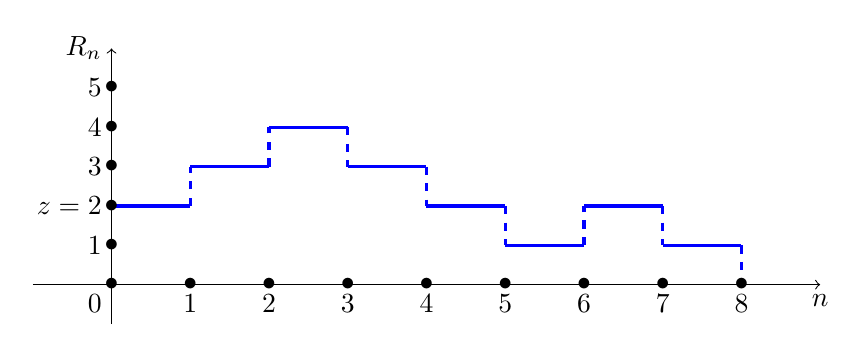
\begin{tikzpicture}
  %Origin and axis
  \coordinate (O) at (0,0);
  \draw[->] (-1,0) -- (9,0) coordinate[label = {below:$n$}] (xmax);
  \draw[->] (0,-0.5) -- (0,3) coordinate[label = {left:$R_n$}] (ymax);
  %Lower linear boundary

 
  %Stochastic process trajectory
  
  \draw (0,0) node[blue,left] {} node{};
  \draw[very thick,blue,-] (0,1) -- (1,1) node[pos=0.5, above] {} ;
  \draw[very thick,dashed,blue] (1,1) -- (1,1.5) node[pos=0.5, right] {};
  \draw[very thick,blue,-] (1,1.5) -- (2,1.5) node[pos=0.5, above] {};
  \draw[very thick,dashed,blue] (2,1.5) -- (2,2) node[pos=0.5, right] {};
  \draw[very thick,blue,-] (2,2) -- (3,2) node[pos=0.5, above] {};
  \draw[very thick,dashed,blue] (3,2) -- (3,1.5) node[pos=0.5, right] {};
  \draw[very thick,blue,-] (3,1.5) -- (4,1.5)node[pos=0.5, above] {};
  \draw[very thick,dashed,blue] (4,1.5) -- (4,1) node[pos=0.5, right] {};  
  \draw[very thick,blue,-] (4,1) -- (5,1) node[pos=0.5, above] {};
  \draw[very thick,dashed,blue] (5,1) -- (5,0.5) node[pos=0.5, right] {};  
  \draw[very thick,blue,-] (5,0.5) -- (6,0.5) node[pos=0.5, above] {};
  \draw[very thick,dashed,blue,-] (6,0.5) -- (6,1) node[pos=0.5, above] {};
   \draw[very thick,blue,-] (6,1) -- (7,1) node[pos=0.5, above] {};
    \draw[very thick,dashed,blue,-] (7,1) -- (7,0.5) node[pos=0.5, above] {};
     \draw[very thick,blue,-] (7,0.5) -- (8,0.5) node[pos=0.5, above] {};
     \draw[very thick,dashed,blue,-] (8,0.5) -- (8,0) node[pos=0.5, above] {};
  %Jump Times
  \draw (1,0) node[black,below] {$1$} node{ \color{black}$\bullet$};
  \draw (2,0) node[black,below] {$2$} node{ \color{black}$\bullet$};
  \draw (3,0) node[black,below] {$3$} node{ \color{black}$\bullet$};
  \draw (4,0) node[black,below] {$4$} node{ \color{black}$\bullet$};
  \draw (5,0) node[black,below] {$5$} node{ \color{black}$\bullet$};
  \draw (6,0) node[black,below] {$6$} node{ \color{black}$\bullet$};
  \draw (7,0) node[black,below] {$7$} node{ \color{black}$\bullet$};
  \draw (8,0) node[black,below] {$8$} node{ \color{black}$\bullet$};
  %Level of the counting process
   \draw (0,0) node[black,below left] {$0$} node{ \color{black}$\bullet$};
   \draw (0,0.5) node[black,left] {$1$} node{ \color{black}$\bullet$};
   \draw (0,1) node[black,left] {$z=2$} node{ \color{black}$\bullet$};
   \draw (0,1.5) node[black,left] {$3$} node{ \color{black}$\bullet$};
   \draw (0,2) node[black,left] {$4$} node{ \color{black}$\bullet$};
   \draw (0,2.5) node[black,left] {$5$} node{ \color{black}$\bullet$};

  % %Aggregated Capital gains
%  \draw (0,1.5) node[blue,below right] {$\mu_1$} node{ \color{blue}$-$};
%  \draw (0,2.25) node[blue,left] {$\mu_2$} node{ \color{blue}$-$};
%  \draw (0,3.75) node[blue,left] {$\mu_3$} node{ \color{blue}$-$};
  %Ruin time = First-crossing time time
%  \draw (5,0) node[black,above right] {${\tau_0}_u$} node{ \color{black}$\times$};
%  \draw[dotted,black] (0,3.28) -- (5,3.28);
%  \draw[dotted,black] (5,0) -- (5,3.28);
\end{tikzpicture}
\end{center}
\caption{Illustration of the first-hitting time problem of a double spending attack.}
\label{fig:double_spending_time}
\end{figure}
Let us denote by 
$$
\mathbb{P}_z(\cdot) = \mathbb{P}(\cdot|R_0 = z)\text{ and }\mathbb{E}_z(\cdot) = \mathbb{E}(\cdot|R_0 = z) 
$$
We are interested for now in the cvonditional distribution of ${\tau_0}$ provided that $R_0 = z$.
\subsubsection{Double spending probability}\label{sssec:double_spending_rw_dsp}
The double spending probability is defined as 
$$
\phi(z)=\mathbb{P}_z({\tau_0} <\infty),
$$
and given in the following result
\begin{theo}
If $p>q$ then 
$$
\phi(z) = \left(\frac{q}{p}\right)^z.
$$
\end{theo}
\noindent We give two proofs for this result, the first one uses simple first step analysis exploiting the Markov property of the random walk. The second one uses Martingale and the optional stopping theorem.\\

\underline{\textit Proof 1:}\\
Using a first step analysis, we have 
\begin{equation}\label{eq:difference_equation}
\phi(z) = p\phi(z+1)+(1-p)\phi(z-1),\text{ }z\geq1.
\end{equation}
We also have the boundary conditions
\begin{equation}\label{eq:boundary_conditions_double_spending}
\phi(0) = 1\text{ and }\underset{z\rightarrow +\infty}{\lim}\phi(z) = 0
\end{equation}
Equation \eqref{eq:difference_equation} is a linear difference equation of order $2$ associated to the following characteristic equation
$$
px^2 - x + 1-p = 0
$$
which has two roots on the real line with 
$$
r_1 = 1, \text{ and }r_2 = \frac{1-p}{p}.
$$
The solution of \eqref{eq:difference_equation} is given by 
$$
\phi(z)=A+B\left(\frac{1-p}{p}\right)^z,
$$
where $A$ and $B$ are constant. Using the boudary conditions \eqref{eq:boundary_conditions_double_spending}, we deduce that
$$
\phi(z) = \left(\frac{1-p}{p}\right)^z
$$
as announced.\\
For the second proof we need the notion of martingale
\begin{definition}
A stochastic process $(X_n)_{n\geq0}$, is called a martingale with respect to a filtration $\mathcal{F}_n$, if
\begin{itemize}
  \item[(i)] $X_n$ is $\mathcal{F}_n$-adapted
  \item[(ii)] $\mathbb{E}(X_n)<\infty\text{ for }n\geq\geq0$ 
  \item[(iii)] $\mathbb{E}(X_n|\mathcal{F}_{n-1}) = X_{n-1}$
\end{itemize} 
\end{definition}
\noindent and the optional stopping theorem.
\begin{theo}
Let $T$ be a stopping time for the Martingale $(X_n)_{n\geq0}$ then it holds that 
$$
\mathbb{E}(X_T) = \mathbb{E}(X_0) 
$$
in each of the following situations
\begin{itemize}
\item[(i)] $T$ is bounded almost surely 
\item[(ii)] There exists $c>0$ such that $|X_{T\land n}|<c$ for every $n>0$.
\item[(iii)] $\mathbb{E}(T)<\infty$, and, for some $K>0$ we have that 
$$
|X_n(\omega) - X_{n-1}(\omega)|\leq K,\text{ }\forall (n,\omega).
$$
\end{itemize}

\end{theo}
\underline{\textit Proof 2:}\\
Define the process 
$$
X_n = \exp\left[sR_n- n\kappa_Y(s)\right],
$$
where $s>0$, and 
$$
\kappa_Y(s) = \log\left[\mathbb{E}\left(e^{sY}\right)\right],
$$
is the cumulant generating function of $Y$. 
\begin{lemma}\label{lem:wald_martingale_RW}
$(X_n)_{n\geq0}$ is a $\mathcal{F}_n$-martingale.
\end{lemma}
\begin{proof}
Denote by $M_Y(s) = \mathbb{E}(e^{sY})$ the moment generating function of $Y$, we have that 
\begin{eqnarray*}
\mathbb{E}(X_n|\mathcal{F}_n)&=&\mathbb{E}\left\{\exp\left[sR_n - n\kappa_Y(s)\right]|\mathcal{F}_n\right\}\\
&=&\exp\left[sR_{n-1} - n\kappa_Y(s)\right]\mathbb{E}\left[\exp\left(sY_{n}\right)|\mathcal{F}_n\right]\\
&=&\exp\left[sR_{n-1} \right]M_Y(s)^{-n} M_Y(s)\\
&=& X_{n-1}.
\end{eqnarray*}
\end{proof} 
The equation $\kappa_Y(s) = 0$ is equivalent to 
$$
pe^s+qe^{-s} = 1
$$
which admits $\gamma =\log(q/p)$ as only nonnegative solution. The process $(\e^{\gamma R_n})_{n\geq0}$ is a $\mathcal{F}_n$-Martingale. Define $\tau_a = \inf\{n\geq 0\text{ ; }R_n = a\}$, for $a>z$. Consider the stopping time $\tau = \tau_0\land\tau_a$, we have that for any $n>0$, 
$$
\mathbb{P}( \tau=\infty) \leq \mathbb{P}( \tau > n) < \mathbb{P}( |R_n| \leq a) = 0;
$$
We can therefore apply the optional stopping time theorem at $\tau$ to get
\begin{eqnarray*}
 \mathbb{E}(X_{\tau}) = \mathbb{E}(X_{0})&\Leftrightarrow& \mathbb{P}(\tau = \tau_0) + [1- \mathbb{P}(\tau = \tau_0)]\e^{a z}= \e^{\gamma z}\\
 &\Leftrightarrow& \mathbb{P}(\tau = \tau_0)] = \frac{\e^{\gamma z}-\e^{a z}}{1-\e^{az}}.
\end{eqnarray*}
We then let $a\rightarrow\infty$ in the above equation to conclude that 
$$
\mathbb{P}(\tau = \tau_0) =\left(\frac{q}{p}\right)^z.
$$
\begin{exercise}
What happens if
\begin{itemize}
\item $p = q = 1/2$? 
\item $q>p$?
\end{itemize}
\end{exercise}
In practice the number of blocks $z$ is actually random variable 
$$
Z = (\alpha -M)_+,
$$ 
where $M$ corresponds to the number of blocks the attacker managed to mine while the vendor waits for $\alpha$ confirmations. If we assume that a block mined by the honest miners is a success while a block mined by the attacker is a failure then $M$ actually counts the number of failure before $\alpha$ successes. We have that $M\sim \text{Neg-Bin}(\alpha, p)$ where $M$ has a probability mass function (\pmf) given by 
$$
\mathbb{P}(M = m) = \binom{\alpha+m-1}{m}p^\alpha q^m.
$$
Whenever $Z = 0$ then double spending occur right away as $\phi(0) =1$. To derive the double spending probability, we condition upon the values of $Z$ via the law of total probability 
$$
\mathbb{P}( \text{Double Spending}) = \mathbb{P}(M\geq \alpha)+\sum_{m = 0}^{\alpha-1}\binom{\alpha+m-1}{m}q^\alpha p^m.
$$
The analysis conducted here is similar to that of \citet{rosenfeld2014analysis}.
\subsubsection{Double spending time}\label{sssec:double_spending_rw_dst}
In the block mining world time is money. Every hour spent in computing hashes is costly in terms of energy. It is then very interesting to know whether a double spending attack is meant to last long or not. Intuitively, we can think that if it must occur the it should at a earlier stage because as $p>1/2$ our random walk $(R_n)_{n\geq0}$ will eventually drift toward $+\infty$. The following result provides the probability distribution of $\tau_0$ when $R_0 = z$.
\begin{theo}
If $z = 0$ then $\tau_0=0$ almost surely. If $z>0$ then $\tau_0$ admits a \pmf given by 
$$
\mathbb{P}_z(\tau_0 = n)=
\frac{z}{n}\binom{n-z}{(n-z) / 2}p^{(n-z) / 2}q^{(n
+z) / 2}\text{ if }n>z\text{ and }n-z\text{ is even},
$$
and $0$ otherwise.
\end{theo}
\begin{proof}
We start by showing the following lemma, sometimes referred to as the Markov hitting time theorem.
\begin{lemma}\label{lem:markov_hitting_time}
\begin{equation}\label{eq:markov_hitting_time}
\mathbb{P}_z(\tau_0 = n) = \frac{z}{n}\mathbb{P}_z(R_n = 0)
\end{equation}
\end{lemma}
\begin{proof}
If $z = 0$ then $\tau_0 = 0$ almost surely and both sides of \eqref{eq:markov_hitting_time} equal to $0$. Assume that $z\geq1$, we have that $\mathbb{P}_z(\tau_0 = n) = 0$ and $\mathbb{P}_z(R_n = 0) = 0$ whenever $n<z$ and $n-z$ is odd. The rest of the proof is by induction on $n\geq1$, when $n = 1$ we have that 
$$
\mathbb{P}_z(\tau_0 = 1) = 0 = \frac{z}{1}\mathbb{P}_z(R_1 = 0),\text{ for }z>1, 
$$
and 
$$\mathbb{P}_1(\tau_0 = 1) = q = \frac{1}{1}\mathbb{P}_1(R_1 = 0),\text{ for }z=1. 
$$
The property holds for $n=1$. Assume that it holds for some $n\geq1$. The law of total probability yields
\begin{eqnarray*}
\mathbb{P}_z(\tau_0 = n+1)&=&\sum_{y\in\{-1,1\}}\mathbb{P}_z(\tau_0 = n+1|Y_1 = y)\mathbb{P}(Y_1 = y)\\
&=&\sum_{y\in\{-1,1\}}\mathbb{P}_{z+y}(\tau_0 = n)\mathbb{P}(Y_1 = y)\\
&=&\sum_{y\in\{-1,1\}}\frac{z+y}{n}\mathbb{P}_{z+y}(R_n = 0)\mathbb{P}(Y_1 = y)
\end{eqnarray*}
The second equality holds thanks to the strong Markov property. We further undo the law of total probability.
\begin{eqnarray}
\mathbb{P}_z(\tau_0 = n+1)&=&\sum_{y\in\{-1,1\}}\frac{z+y}{n}\mathbb{P}_{z}(Y_1 = y|R_{n+1} = 0)\mathbb{P}_z(R_{n+1} = 0)\nonumber\\
&=&\frac{\mathbb{P}_z(R_{n+1} = 0)}{n}\left[z+\mathbb{E}(Y_1|R_{n+1}=0)\right]\label{eq:law_total_probability_undone}
\end{eqnarray}
Since the $Y_i$ are \iid then it holds that 
$$
\mathbb{E}(Y_1|R_{n+1}=0) = \mathbb{E}(Y_i|R_{n+1}=0)\text{, } i = 1, \ldots, n+1,
$$
and it follows that 
$$
\mathbb{E}(Y_1|R_{n+1}=0) = \frac{1}{n+1}\sum_{i =1}^{n+1}\mathbb{E}(Y_i|R_{n+1}=0) = \frac{-z}{n+1}.
$$
Inserting the above expression in \eqref{eq:law_total_probability_undone} yields 
$$
\mathbb{P}_z(\tau_0 = n+1) = \frac{z}{n+1}\mathbb{P}_z(R_{n+1} = 0).
$$
\end{proof}
\begin{remark}
This proof is direct, simple and inspired from \citet{Hofstad2008}. It is possible to make it shorter taking advantage of the ballot theorem. Indeed consider again the first hitting problem on \cref{fig:double_spending_time} and reverse the timeline. It corresponds to that of a random walk $(S_n)_{n\geq0}$ that starts at $0$, make upward jumps with probability $q$, and aims at reaching the level $z$ without crossing the $X$ axis, see \cref{fig:time_reversed_double_spending_time}.
\begin{figure}[ht!]
\begin{center}
 \subfloat[Original first hitting problem]
 {
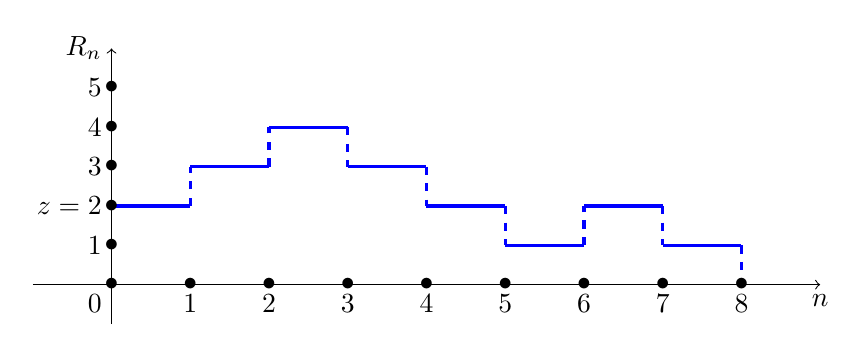
\begin{tikzpicture}
  %Origin and axis
  \coordinate (O) at (0,0);
  \draw[->] (-1,0) -- (9,0) coordinate[label = {below:$n$}] (xmax);
  \draw[->] (0,-0.5) -- (0,3) coordinate[label = {left:$R_n$}] (ymax);
  %Lower linear boundary

 
  %Stochastic process trajectory
  
  \draw (0,0) node[blue,left] {} node{};
  \draw[very thick,blue,-] (0,1) -- (1,1) node[pos=0.5, above] {} ;
  \draw[very thick,dashed,blue] (1,1) -- (1,1.5) node[pos=0.5, right] {};
  \draw[very thick,blue,-] (1,1.5) -- (2,1.5) node[pos=0.5, above] {};
  \draw[very thick,dashed,blue] (2,1.5) -- (2,2) node[pos=0.5, right] {};
  \draw[very thick,blue,-] (2,2) -- (3,2) node[pos=0.5, above] {};
  \draw[very thick,dashed,blue] (3,2) -- (3,1.5) node[pos=0.5, right] {};
  \draw[very thick,blue,-] (3,1.5) -- (4,1.5)node[pos=0.5, above] {};
  \draw[very thick,dashed,blue] (4,1.5) -- (4,1) node[pos=0.5, right] {};  
  \draw[very thick,blue,-] (4,1) -- (5,1) node[pos=0.5, above] {};
  \draw[very thick,dashed,blue] (5,1) -- (5,0.5) node[pos=0.5, right] {};  
  \draw[very thick,blue,-] (5,0.5) -- (6,0.5) node[pos=0.5, above] {};
  \draw[very thick,dashed,blue,-] (6,0.5) -- (6,1) node[pos=0.5, above] {};
   \draw[very thick,blue,-] (6,1) -- (7,1) node[pos=0.5, above] {};
    \draw[very thick,dashed,blue,-] (7,1) -- (7,0.5) node[pos=0.5, above] {};
     \draw[very thick,blue,-] (7,0.5) -- (8,0.5) node[pos=0.5, above] {};
     \draw[very thick,dashed,blue,-] (8,0.5) -- (8,0) node[pos=0.5, above] {};
  %Jump Times
  \draw (1,0) node[black,below] {$1$} node{ \color{black}$\bullet$};
  \draw (2,0) node[black,below] {$2$} node{ \color{black}$\bullet$};
  \draw (3,0) node[black,below] {$3$} node{ \color{black}$\bullet$};
  \draw (4,0) node[black,below] {$4$} node{ \color{black}$\bullet$};
  \draw (5,0) node[black,below] {$5$} node{ \color{black}$\bullet$};
  \draw (6,0) node[black,below] {$6$} node{ \color{black}$\bullet$};
  \draw (7,0) node[black,below] {$7$} node{ \color{black}$\bullet$};
  \draw (8,0) node[black,below] {$8$} node{ \color{black}$\bullet$};
  %Level of the counting process
   \draw (0,0) node[black,below left] {$0$} node{ \color{black}$\bullet$};
   \draw (0,0.5) node[black,left] {$1$} node{ \color{black}$\bullet$};
   \draw (0,1) node[black,left] {$z=2$} node{ \color{black}$\bullet$};
   \draw (0,1.5) node[black,left] {$3$} node{ \color{black}$\bullet$};
   \draw (0,2) node[black,left] {$4$} node{ \color{black}$\bullet$};
   \draw (0,2.5) node[black,left] {$5$} node{ \color{black}$\bullet$};

  % %Aggregated Capital gains
%  \draw (0,1.5) node[blue,below right] {$\mu_1$} node{ \color{blue}$-$};
%  \draw (0,2.25) node[blue,left] {$\mu_2$} node{ \color{blue}$-$};
%  \draw (0,3.75) node[blue,left] {$\mu_3$} node{ \color{blue}$-$};
  %Ruin time = First-crossing time time
%  \draw (5,0) node[black,above right] {${\tau_0}_u$} node{ \color{black}$\times$};
%  \draw[dotted,black] (0,3.28) -- (5,3.28);
%  \draw[dotted,black] (5,0) -- (5,3.28);
\end{tikzpicture}
\label{subfig:ds_RW_time}
}
\hskip1em
\subfloat[Time reversed first hitting problem]{
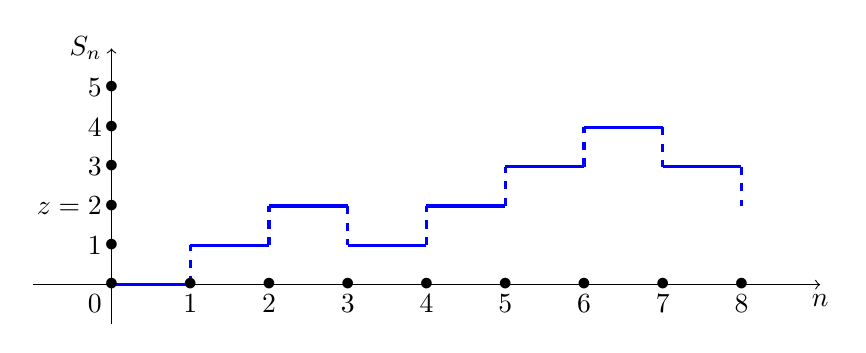
\begin{tikzpicture}
  %Origin and axis
  \coordinate (O) at (0,0);
  \draw[->] (-1,0) -- (9,0) coordinate[label = {below:$n$}] (xmax);
  \draw[->] (0,-0.5) -- (0,3) coordinate[label = {left:$S_n$}] (ymax);
  %Lower linear boundary

 
  %Stochastic process trajectory
  
  \draw (0,0) node[blue,left] {} node{};
  \draw[very thick,blue,-] (0,0) -- (1,0) node[pos=0.5, above] {} ;
  \draw[very thick,dashed,blue] (1,0) -- (1,0.5) node[pos=0.5, right] {};
  \draw[very thick,blue,-] (1,0.5) -- (2,0.5) node[pos=0.5, above] {};
  \draw[very thick,dashed,blue] (2,0.5) -- (2,1) node[pos=0.5, right] {};
  \draw[very thick,blue,-] (2,1) -- (3,1) node[pos=0.5, above] {};
  \draw[very thick,dashed,blue] (3,1) -- (3,0.5) node[pos=0.5, right] {};
  \draw[very thick,blue,-] (3,0.5) -- (4,0.5)node[pos=0.5, above] {};
  \draw[very thick,dashed,blue] (4,0.5) -- (4,1) node[pos=0.5, right] {};  
  \draw[very thick,blue,-] (4,1) -- (5,1) node[pos=0.5, above] {};
  \draw[very thick,dashed,blue] (5,1) -- (5,1.5) node[pos=0.5, right] {};  
  \draw[very thick,blue,-] (5,1.5) -- (6,1.5) node[pos=0.5, above] {};
  \draw[very thick,dashed,blue,-] (6,1.5) -- (6,2) node[pos=0.5, above] {};
   \draw[very thick,blue,-] (6,2) -- (7,2) node[pos=0.5, above] {};
    \draw[very thick,dashed,blue,-] (7,2) -- (7,1.5) node[pos=0.5, above] {};
     \draw[very thick,blue,-] (7,1.5) -- (8,1.5) node[pos=0.5, above] {};
     \draw[very thick,dashed,blue,-] (8,1.5) -- (8,1) node[pos=0.5, above] {};
  %Jump Times
  \draw (1,0) node[black,below] {$1$} node{ \color{black}$\bullet$};
  \draw (2,0) node[black,below] {$2$} node{ \color{black}$\bullet$};
  \draw (3,0) node[black,below] {$3$} node{ \color{black}$\bullet$};
  \draw (4,0) node[black,below] {$4$} node{ \color{black}$\bullet$};
  \draw (5,0) node[black,below] {$5$} node{ \color{black}$\bullet$};
  \draw (6,0) node[black,below] {$6$} node{ \color{black}$\bullet$};
  \draw (7,0) node[black,below] {$7$} node{ \color{black}$\bullet$};
  \draw (8,0) node[black,below] {$8$} node{ \color{black}$\bullet$};
  %Level of the counting process
   \draw (0,0) node[black,below left] {$0$} node{ \color{black}$\bullet$};
   \draw (0,0.5) node[black,left] {$1$} node{ \color{black}$\bullet$};
   \draw (0,1) node[black,left] {$z=2$} node{ \color{black}$\bullet$};
   \draw (0,1.5) node[black,left] {$3$} node{ \color{black}$\bullet$};
   \draw (0,2) node[black,left] {$4$} node{ \color{black}$\bullet$};
   \draw (0,2.5) node[black,left] {$5$} node{ \color{black}$\bullet$};

  % %Aggregated Capital gains
%  \draw (0,1.5) node[blue,below right] {$\mu_1$} node{ \color{blue}$-$};
%  \draw (0,2.25) node[blue,left] {$\mu_2$} node{ \color{blue}$-$};
%  \draw (0,3.75) node[blue,left] {$\mu_3$} node{ \color{blue}$-$};
  %Ruin time = First-crossing time time
%  \draw (5,0) node[black,above right] {${\tau_0}_u$} node{ \color{black}$\times$};
%  \draw[dotted,black] (0,3.28) -- (5,3.28);
%  \draw[dotted,black] (5,0) -- (5,3.28);
\end{tikzpicture}
\label{subfig:time_reversed_ds_RW_time}
}
\end{center}
\caption{Another look at the first hitting time problem.}
\label{fig:time_reversed_double_spending_time}
\end{figure}
Note that \cref{subfig:time_reversed_ds_RW_time} is the reflection of \cref{subfig:ds_RW_time} with respect to the $Y$ axis. We have equivalently
$$
\mathbb{P}_z(\tau_0) = \mathbb{P}(S_k>0,\text{ }1\leq k\leq n|S_n = z, S_0 = 0)\mathbb{P}_0(S_n = z|S_0=0),
$$
and 
$$
\mathbb{P}(S_k>0,\text{ }1\leq k\leq n|S_n = z, S_0 = 0) = \frac{z+(n-z)/2-(n-z)/2}{n} = \frac{z}{n}.
$$
For proof of the ballot theorem, see \citet{Renault2007}. For a general formulation and application to queueing see \citet{Takacs1962}.
\end{remark}
To complete the proof, we just note that 
$$
\mathbb{P}_z(R_n = 0) = \binom{n-z}{(n-z) / 2}p^{(n-z) / 2}q^{(n
+z) / 2}
$$
as it corresponds to a trajectory of $(R_n)_{n \geq0}$ starting at $R_0 = z$ ending at $0$ made of $(n-z)/2$ upward jumps and $(n+z)/2$ downward one.
\end{proof}
Just like in the previous section, the actual double spending time depends on the value of the random variable $Z = (\alpha -M)_+$.

\subsection{Counting process model}\label{sec:counting_process}
Our aim is to go from the discrete time framework of the previous section to a continuous time. To do so, we will model the length of the blockchain as counting processes. We will consider renewal processes and more specifically Poisson processes. We start by giving some reminders on the exponential distribution and counting processes before studying the double spending time distribution.

\subsubsection{Poisson process, Exponential distributions and friends}\label{sssec:exp_distribution}
\begin{definition}\label{def:counting_process}
A counting process $(N_t)_{t\geq0}$ is a continuous time stochastic process that counts the occurence of an event over time such that
\begin{equation*}
N_0=0\text{ and }N_t=\sum_{k=1}^{+\infty}\mathbb{I}_{T_k\leq t}.
\end{equation*}
where $T_1,T_2,T_3,\ldots$ denote the arrival times, with the convention that $T_0=0$. Let $\Delta^T_0,\Delta^T_1,\Delta^T_2,\ldots$ be the sequence of inter-arrival times defined as
$$
\Delta^T_k=T_{k+1}-T_{k}\text{, }k=0,1,2\ldots.
$$
\end{definition}
A trajectory of a counting process is given in 
\begin{figure}[!h]
\begin{center}
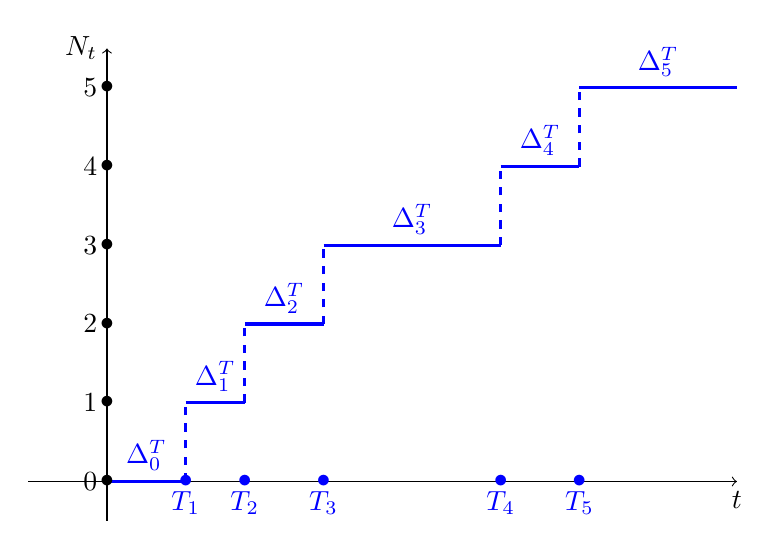
\begin{tikzpicture}[scale=1]
  %Origin and axis
  \coordinate (O) at (0,0);
  \draw[->] (-1,0) -- (8,0) coordinate[label = {below:$t$}] (xmax);
  \draw[->] (0,-0.5) -- (0,5.5) coordinate[label = {left:$N_t$}] (ymax);
  %Lower linear boundary


  %Stochastic process trajectory

  \draw (0,0) node[blue,left] {} node{};
  \draw[very thick,blue,-] (0,0) -- (1,0) node[pos=0.5, above] {$\Delta^T_0$} ;
  \draw[very thick,dashed,blue] (1,0) -- (1,1) node[pos=0.5, right] {};
  \draw[very thick,blue,-] (1,1) -- (1.75,1) node[pos=0.5, above] {$\Delta^T_1$};
  \draw[very thick,dashed,blue] (1.75,1) -- (1.75,2) node[pos=0.5, right] {};
  \draw[very thick,blue,-] (1.75,2) -- (2.75,2) node[pos=0.5, above] {$\Delta^T_2$};
  \draw[very thick,dashed,blue] (2.75,2) -- (2.75,3) node[pos=0.5, right] {};
  \draw[very thick,blue,-] (2.75,3) -- (5,3)node[pos=0.5, above] {$\Delta^T_3$};
  \draw[very thick,dashed,blue] (5,3) -- (5,4) node[pos=0.5, right] {};
  \draw[very thick,blue,-] (5,4) -- (6,4) node[pos=0.5, above] {$\Delta^T_4$};
  \draw[very thick,dashed,blue] (6,4) -- (6,5) node[pos=0.5, right] {};
  \draw[very thick,blue,-] (6,5) -- (8,5) node[pos=0.5, above] {$\Delta^T_5$};
  %Jump Times
  \draw (1,0) node[blue,below] {$T_1$} node{ \color{blue}$\bullet$};
  \draw (1.75,0) node[blue,below] {$T_2$} node{ \color{blue}$\bullet$};
  \draw (2.75,0) node[blue,below] {$T_3$} node{ \color{blue}$\bullet$};
  \draw (5,0) node[blue,below] {$T_4$} node{ \color{blue}$\bullet$};
  \draw (6,0) node[blue,below] {$T_5$} node{ \color{blue}$\bullet$};
  %Level of the counting process
   \draw (0,0) node[black,left] {$0$} node{ \color{black}$\bullet$};
   \draw (0,1) node[black,left] {$1$} node{ \color{black}$\bullet$};
   \draw (0,2) node[black,left] {$2$} node{ \color{black}$\bullet$};
   \draw (0,3) node[black,left] {$3$} node{ \color{black}$\bullet$};
   \draw (0,4) node[black,left] {$4$} node{ \color{black}$\bullet$};
   \draw (0,5) node[black,left] {$5$} node{ \color{black}$\bullet$};
\end{tikzpicture}
\end{center}
\caption{Trajectory of the counting process $(N_t)_{t\geq0}$.}
\label{fig:trajectory_counting_process}
\end{figure}
\begin{definition}\label{def_poisson_process}
A Poisson process $(N_t)_{t\geq0}$ is a conting process whose inter-arrival times are \iid exponential random variables.
\end{definition}
\begin{definition}\label{def:exp_dist}
A random variable $X$ is exponentially distributed $X\sim\ExpDist(\lambda)$ if it has \pdf
$$
f_X(x) =\begin{cases} 
\lambda\e^{-\lambda x},&\text{ if }x>0,\\
0,&\text{ otherwise}.
\end{cases}
$$
\end{definition}
For some reasons, we need to introduce the joint distribution of the order statistics of a uniform random sample.
\begin{prop}\label{def:uniform_OS_dist}
Let $U_1,\ldots, U_n$ be a sample of \iid uniform random variables on $(a,b)$. Denote by 
$$
U_{(1)}\leq U_{(2)}\leq\ldots\leq U_{(n)}
$$
the order statistics of such a sample. The joint distribution of $(U_{(1)},\ldots,  U_{(n)})$ is given by 
$$
f_{(U_{(1)},\ldots, U_{(n)})}(u_1,\ldots, u_n)=\frac{n!}{(b-a)^n}\mathbb{I}_{a<u_1<\ldots< u_n<b}(u_1,\ldots, u_n).
$$
and we denote $(U_{(1)},\ldots,  U_{(n)})\sim \text{OS}_n([a,b])$
\end{prop}
\begin{proof}
Let $g:\mathbb{R}^n\mapsto \mathbb{R}_+$ be measurable and bounded. We have that
$$
\mathbb{E}[g(U_{(1)},\ldots,U_{(n)})]=\mathbb{E}\left[\sum_{\sigma\in\mathcal{S}_n}
g(U_{\sigma(1)},\ldots,U_{\sigma(n)})
\mathbb{I}_{U_{\sigma(1)} <\ldots< U_{\sigma(n)}}
\right]
$$
where $\mathcal{S}_n$ the set of all the permutation of $\{1,\ldots,n \}$. We note that
\begin{eqnarray*}
\mathbb{E}\left[g(U_{\sigma(1)},\ldots,U_{\sigma(n)})
\mathbb{I}_{U_{\sigma(1)} <\ldots< U_{\sigma(n)}}
\right]&=& \mathbb{E}\left[g(U_{1},\ldots,U_{n})
\mathbb{I}_{U_{1} <\ldots< U_{n}}\right]\\
&=&\int_{\mathbb{R}^{n}}g(u_{1},\ldots,u_{n})
\mathbb{I}_{u_{1} <\ldots< u_{n}}\frac{1}{(b-a)^n}\text{d}\lambda_{n}(u_1,\ldots, u_n).
\end{eqnarray*}
It then follows that
$$
\mathbb{E}[g(U_{(1)},\ldots,U_{(n)})]=\int_{\mathbb{R}^{n}}g(u_{1},\ldots,u_{n})
\mathbb{I}_{u_{1} <\ldots< u_{n}}\frac{n!}{(b-a)^n}\text{d}\lambda_{n}(u_1,\ldots, u_n).
$$
\end{proof}
We require some additional result about the gamma distribution.
\begin{prop}\label{prop:erlang_dist}
Let $\Delta^T_1,\ldots, \Delta^T_n$ be \iid exponential $\text{Exp}(\lambda)$ random variables, define the sequence $T_k=\sum_{i=1}^{k}\Delta^T_i, k=1,\ldots, n$.
\begin{enumerate}
\item The $T_{k}$'s have an Erlang distribution. We denote by $T_{k}\sim\text{Erl}(k,\lambda)$ with 
$$
f_{T_k}(t)=\frac{t^{k-1}e^{-\lambda t}\lambda^k}{(k-1)!},\text{ }t>0.
$$
\item The joint distribution of $(T_1,\ldots, T_n)$ has \pmf given by
$$
f_{(T_1,\ldots, T_n)}(t_1,\ldots, t_n)=\lambda^n e^{-\lambda t_n }\mathbb{I}_{0<t_1<\ldots< t_n}(t_1,\ldots, t_n)
$$
\item $[(T_1,\ldots, T_n)|T_{n+1}=t]\sim \text{OS}_{n}([0,t])$
\end{enumerate}
\end{prop}
\begin{proof}
\begin{enumerate}
\item We use induction on $k\geq1$. For $k=1$ we have that $\Delta^T_1= T_1$ so the property holds. Assume that the property hold true for some $k$ and consider $k+1$. We note that $T_{k+1}=T_k+\Delta^T_{k+1}$ then
\begin{eqnarray*}
f_{T_{k+1}}(t)&=&\int_{0}^{t}f_{T_k}(x)f_{\Delta^T_{k+1}}(t-x)\text{d}x\\
&=&\int_{0}^{t}\frac{x^{k-1}e^{-\lambda x}\lambda^k}{(k-1)!}\lambda e^{-\lambda(t-x)}\text{d}x\\
&=&\frac{e^{-\lambda t}\lambda^{k+1}}{(k-1)!}\frac{t^k}{k}=\frac{t^k e^{-\lambda t}\lambda^{k+1}}{k!}.
\end{eqnarray*}
\begin{exercise}
Can you propose another way to show this result? Without using induction.
\end{exercise}
\item Let $g:\mathbb{R}^n\mapsto \mathbb{R}_+$ be meaurable and bounded, we have
\begin{eqnarray*}
\mathbb{E}[g(T_{1},\ldots,T_n)]&=& \mathbb{E}[g(\Delta^T_{1},\Delta^T_1+\Delta^T_2\ldots,\Delta^T_1+\ldots+ \Delta^T_n)]\\
&=&\int_{\mathbb{R}^n}g(t_{1},\ldots,t_1+\ldots+ t_n)f_{(\Delta^T_{1},\ldots,\Delta^T_n)}(t_1,\ldots,t_n)\text{d}\lambda_n(t_{1},\ldots,t_n)\\
\end{eqnarray*}
Let us apply the following change of variable 
$$
\Phi:(u_{1},\ldots,u_n)\mapsto(u_1, u_{2}-u_1,\ldots,u_n-u_{n-1}):=(t_1,\ldots, t_n),$$
minding the change in the integration domain as 
$$
\Phi(\mathbb{R}_+\times ]u_1,\infty[\times \ldots\times ]u_{n-1},\infty[) = \mathbb{R}^n 
$$
and the Jacobian $\left|\frac{\text{d}\Phi}{\text{d}u}\right|=1$. It follows that
$$
\mathbb{E}[g(T_{1},\ldots,T_n)]=\int_{\mathbb{R}^n} g(u_1,\ldots, u_n)\lambda^{n}e^{-\lambda u_n}\mathbb{I}_{0<u_1<\ldots<u_n}(u_1,\ldots, u_n)\text{d}\lambda_{n}(u_1,\ldots, u_n).
$$
\item We have that 
\begin{eqnarray*}
f_{T_1,\ldots, T_n|T_{n+1}}(t_1,\ldots,t_n|t)
&=&\frac{f_{T_1,\ldots, T_n,T_{n+1}}(t_1,\ldots,t_n,t)}{f_{T_{n+1}(t)}}\\
&=&\frac{n!}{t^n}\mathbb{I}_{0<t_1<\ldots< t_n<t}(t_1,\ldots, t_n, t).
\end{eqnarray*}
\end{enumerate}
\end{proof}
The fact that the Poisson process is a Levy process will be useful later on, so here it is
\begin{prop}
The following statements are equivalent
\begin{enumerate}
\item $(N_t)_{t\geq 0}$ is a Poisson process
\item The stochastic process $(N_t)_{t\geq 0}$ has
\begin{itemize}
\item[(i)] independent increments, it means that for $0<t_1\leq\ldots\leq t_n$, the random variables
$N_{t_1},N_{t_2}-N_{t_1},\ldots,N_{t_{n}}-N_{t_{n-1}}$
are independent.
\item[(ii)] stationnary increments in the sense that the event frequency distribution over some time period of duration $s>0$ only depends on $s$. Indeed, we have that 
$$
N_{t+s}-N_t\sim\PoissonDist(\lambda s),\text{ for }s,t\geq 0.
$$
\end{itemize}
\end{enumerate}
The stochastic processes with independent and stationnary increments are called Levy processes.
\end{prop}
\begin{proof}
\underline{$1 \Rightarrow 2$}\\
Assume that $(N_t)_{t\geq0}$ is a Poisson process and let $0<t_1<\ldots <t_n$ be some times. Consider the folowing probability 
$$
\mathbb{P}\left(N_{t_1} = j_1, N_{t_2}-N_{t_1} = j_2,\ldots, N_{t_n}-N_{t_{n-1}} = j_n\right)
$$
such that $j_1,\ldots, j_n\in \mathbb{N}$. We can rewrite it as 
$$
\mathbb{P}\left(T_{k_1}\leq t_1<T_{k_1+1}, T_{k_2}\leq t_2<T_{k_2+1},\ldots, T_{k_n} \leq t_n<T_{k_n+1}\right),
$$
where $k_i = j_1 + \ldots +j_i, i = 1,\ldots, n$. Conditionning with respect to  $T_{k_n+1}$ yields
\begin{eqnarray*}
&&\mathbb{P}\left(T_{k_1}\leq t_1<T_{k_1+1}, T_{k_2}\leq t_2<T_{k_2+1},\ldots, T_{k_n}\leq t_n<T_{k_n+1}\right)\\
&=&\int_{t_n}^{+\infty}\mathbb{P}\left(T_{k_1}<t_1<T_{k_1+1}, T_{k_2}<t_2<T_{k_2+1},\ldots, T_{k_n}<t_n|T_{k_n +1}=t\right)f_{T_{k_n+1}}(t)\text{d}\lambda(t)\\
&=& \int_{t_n}^{+\infty}\binom{k_n}{j_1,\ldots, j_n}\left(\frac{t_1}{t}\right)^{j_1}\left(\frac{t_2-t_1}{t}\right)^{j_2}\ldots \left(\frac{t_n-t_{n-1}}{t}\right)^{j_n}\frac{e^{-\lambda t}t^{k_n}\lambda^{k_n + 1}}{k_n!}\text{d}\lambda(t)\\
&=&\frac{e^{-\lambda t_1}\left(t_1\right)^{j_1}}{j_1!}\frac{\left(t_2-t_1\right)^{j_2}e^{-\lambda(t_2 - t_1)}}{j_2!}\ldots \frac{\left(t_n-t_{n-1}\right)^{j_n}e^{-\lambda(t_n - t_{n-1})}}{j_n!}
\end{eqnarray*}
From the second to the third equality we simply ask that amomg $k_n$ uniform random variables $j_1$ fall inside $(0,t_1)$, $j_2$ fall inside $(t_1,t_2)$, etc...


\noindent \underline{$2 \Rightarrow 1$}\\
We aim at showing that $(T_1,\ldots, T_n)$ has \pdf given by
\begin{equation}\label{eq:joint_density_arrival_times}
f_{T_1,\ldots, T_n}(t_1,\ldots, t_n)=\lambda^n e^{-\lambda t_n}\mathbb{I}_{0< t_1<\ldots<t_n}.
\end{equation}
Let $t_1,\ldots, t_n$ and $h$ be nonnegative real numbers such that
$$
t_1<t_1+h<t_2<\ldots<t_n<t_n+h,
$$ 
We have
\begin{eqnarray*}
&&\mathbb{P}(t_1<T_1<t_1+h,\ldots,t_n<T_1<t_n+h)\\
&=&\mathbb{P}(N_{t_1}=0,N_{t_1+h}-N_{t_1}=1,\ldots,N_{t_n}-N_{t_{n-1}+h}=0,N_{t_n+h}-N_{t_n}\geq 1)\\
&=&e^{-\lambda t_1}e^{-\lambda h}\lambda h e^{-\lambda [t_2-(t_1+h)]}e^{-\lambda h}\lambda h\ldots e^{-\lambda [t_n-(t_{n-1}+h)]}[1-e^{-\lambda h}] \\
&=&e^{-\lambda t_n}\lambda^{n-1}h^{n-1}[1-e^{-\lambda h}]\\
\end{eqnarray*}
Divide by $h^{n}$ and let $h$ go to $0$ to get \eqref{eq:joint_density_arrival_times}. After applying a change of variable (reciprocal of that used in the proof of \cref{prop:erlang_dist}) to recover the joint distribution of $(\Delta^{T}_1, \ldots, \Delta^{T}_n)$, we see that the later is actually that of an \iid sample of size $n$ of exponential random variables.
\end{proof}
Last but not the lis, we establish the order statistic property of the Poisson process.
\begin{prop}
Provided that$\{N_t=n\}$, The jump times $T_1,\ldots,T_n$ have the same distribution as the order statistic of an \iid sample of $n$ uniform random variable on $(0,t)$, namely it holds that
$$
[T_1,\ldots,T_n|N_t=n]\sim \left(U_{(1)}(0,t),\ldots, U_{(n)}(0,t)\right).
$$
\end{prop}
\begin{proof}
We have
\begin{eqnarray*}
&&\mathbb{E}\left[g(T_1,\ldots, T_n)|N_t = n\right]\\
&=&\frac{\mathbb{E}\left[g(T_1,\ldots, T_n)\mathbb{I}_{N_t = n}\right]}{\mathbb{P}(N_t = n)}\\
&=&\frac{n!}{e^{-\lambda t}(\lambda t)^n}\int_{\mathbb{R}^{n+1}}g(t_1,\ldots, t_n)\mathbb{I}_{t_n\leq t<t_{n+1}}(t_n,t_{n+1})f_{T_1,\ldots, T_{n+1}}(t_1,\ldots, t_{n+1})\text{d}\lambda_{n+1}(t_1,\ldots, t_{n+1})\\
&=&\frac{n!}{e^{-\lambda t}(\lambda t)^n}\int_{\mathbb{R}^{n}}\int_{t}^{+\infty}g(t_1,\ldots, t_n)\mathbb{I}_{0<t_1<\ldots t_n\leq t}(t_1,\ldots,t_{n})\lambda^{n+1} e^{-\lambda t_{n+1}}\text{d}\lambda_{n+1}(t_1,\ldots, t_{n+1})\\
&=&\frac{n!}{e^{-\lambda t}(\lambda t)^n}\int_{\mathbb{R}^{n}}\int_{t}^{+\infty}g(t_1,\ldots, t_n)\mathbb{I}_{0<t_1<\ldots t_n\leq t}(t_1,\ldots,t_{n})\lambda^{n} \text{d}\lambda_{n}(t_1,\ldots,t_n)\e^{-\lambda t}\\
 &=&\int_{\mathbb{R}^{n}}g(t_1,\ldots, t_n)\frac{n!}{t^n}\mathbb{I}_{0<t_1<\ldots t_n\leq t}(t_1,\ldots,t_{n})\text{d}\lambda(t_1,\ldots,t_{n} ).
\end{eqnarray*}
\end{proof}
\noindent The order statistic property of the Poisson process will be useful to solve the first hitting time problem arising later on. To fully benefit from this nice property, we need to introduce Appell and Abel-Gontcharov polynomials.\\

\noindent Let $U=\{u_i, \, i\geq 1\}$ be a non-decreasing sequence of real numbers. To $U$ is attached a (unique) family of Appell polynomials of degree $n$ in $x$, $\{A_{n}(x\vert U),\, n\geq 0\}$ defined as follows.
\begin{definition} 
Starting with $A_0(x\vert U)=1$, the $A_n(x\vert U)$'s satisfy the differential equations
\begin{equation}\label{eq:DifferentialEquationAppellPolynomial}
A_{n}^{(1)}(x|U)=nA_{n-1}(x|U),  
\end{equation}
with the border conditions
\begin{equation}\label{eq:Border AppellPolynomial}
A_{n}(u_{n}|U)=0, \quad n\geq 1.
\end{equation}
So, each $A_n$ has the integral representation
\begin{equation}\label{eq:IntegralRepresentationAppellPolynomials}
A_{n}(x|U)=n!\int_{u_{n}}^{x}\left[\int_{u_{n-1}}^{y_{n}}\text{d}y_{n-1} \ldots \int_{u_{1}}^{y_{1}}\text{d}y_{1}\right]\text{d}y_{n}, \quad n\geq 1.
\end{equation}
\end{definition}

In parallel, to $U$ is attached a (unique) family of Abel-Gontcharov (A-G) polynomials of degree $n$ in $x$, $\{G_{n}(x\vert U),\, n\geq 0\}$.
\begin{definition} 
Starting with $G_0(x\vert U)=1$, the $G_n(x\vert U)$'s satisfy the differential equations
\begin{equation}\label{eq:DifferentialEquationAGPolynomials}
G_n^{(1)}(x|U)=nG_{n-1}(x|{\cal E}U), 
\end{equation}
where ${\cal E}U$ is the shifted family $\{u_{i+1}, \, i\geq 1\}$, and with the border conditions
\begin{equation}\label{eq:Border AGPolynomial}
G_{n}(u_{1}|U)=0, \quad  n\geq 1.
\end{equation}
So, each $G_n$ has the integral representation
\begin{equation}\label{eq:IntegralRepresentationAGPolynomials}
G_{n}(x|U)=n!\int_{u_{1}}^{x}\left[\int_{u_{2}}^{y_{1}}\text{d}y_{2} \ldots \int_{u_{n}}^{y_{n-1}}\text{d}y_{n}\right]\text{d}y_{1}, \quad n\geq 1.
\end{equation}
\end{definition}
\noindent The Appell and A-G polynomials are closely related through the identity
\begin{equation}\label{eq:DefinitionAGPolynomials}
G_{n}(x|u_{1},\ldots,u_{n})=A_{n}(x|u_{n},\ldots,u_{1}), \quad n\geq 1.
\end{equation}
The two families (i.e. for all $n\geq 0$), however, are distinct and enjoy different properties. From \eqref{eq:IntegralRepresentationAppellPolynomials} and \eqref{eq:IntegralRepresentationAGPolynomials}, it is clear that the polynomials $A_n$ and $G_n$ can be interpreted in terms of the joint distribution of the vector $(U_{1:n},\ldots,U_{n:n})$. 
\begin{prop}
For $0\leq u_1 \leq \ldots \leq u_{n} \leq x \leq 1$,
\begin{equation}\label{eq:ProbabilisticInterpretationAppellPolynomials}
P[U_{1:n} \geq u_1, \ldots, U_{n:n} \geq u_{n}\, \mbox{ and }\, U_{n:n}\leq x]= 
A_n(x \vert u_1, \ldots, u_{n}), \quad n\geq1.
\end{equation}
For $0\leq x \leq u_1 \leq \ldots \leq u_{n} \leq 1$,
\begin{equation}\label{eq:ProbabilisticInterpretationAGPolynomials}
P[U_{1:n} \leq u_1, \ldots, U_{n:n} \leq u_{n}\, \mbox{ and }\, U_{1:n}\geq x]
= (-1)^n \, G_n(x \vert u_1, \ldots, u_{n}), \quad n\geq 1.
\end{equation}
\end{prop}
The representations \eqref{eq:ProbabilisticInterpretationAppellPolynomials} and \eqref{eq:ProbabilisticInterpretationAGPolynomials} will play a key role for solving first-hitting problem that involve Poisson processes. Numerically, it will be necessary to evaluate some special values of the polynomials. To this end, it is convenient to use the following recusive relations. 
\begin{prop} 
The Appell polynomials are computed through the expansion
\begin{equation}\label{eq:appell_polynomials_recursion_1}
A_{n}(x|U)=\sum_{k=0}^{n}\binom{n}{k}A_{n-k}(0|U)x^{k}, \quad n\geq 1,
\end{equation}
where the $A_{n}(0|U)$'s are obtained recursively from 
\begin{equation}\label{eq:appell_polynomials_recursion_2}
A_{n}(0|U)=-\sum_{k=1}^{n} \binom{n}{k} A_{n-k}(0|U)u_{n}^{k}, \quad n\geq1.
\end{equation}
The A-G polynomials are computed through the recursion
\begin{equation}\label{eq:recursion_AG_polynomials}
G_{n}(x|U)=x^{n}-\sum_{k=0}^{n-1} \binom{n}{k} u_{k+1}^{n-k} G_{k}(x|U), \quad n\geq 1.
\end{equation}
\end{prop}
\begin{proof}
The Maclaurin expansion of $A_n(x|U)$ gives \eqref{eq:appell_polynomials_recursion_1} as
$$
A_n(x|U) = \sum_{k = 0}^n\frac{A_n^{(k)}(x|U)}{k!}x^k = \sum_{k = 0}^n\binom{n}{k}A_{n-k}(x|U)x^k.
$$
Evaluation at $x = u_n$ then provides \eqref{eq:appell_polynomials_recursion_2}. Regarding \eqref{eq:recursion_AG_polynomials}, first note that 
$$
G_n^{(k)}(u_{k+1}|U) = \begin{cases}
1,&\text{ if }k = n,\\
0,&\text{ otherwise.}
\end{cases}
$$
Any polynomials $R(x)$ of degree $n$ can therefore be written as 
$$
R(x)=\sum_{k = 0}^n\frac{R^{(k)}(u_{k+1})}{k!}G_k(x|U).
$$
By expanding $x^n$ one gets \eqref{eq:recursion_AG_polynomials}.
\end{proof}
Hereafter are a couple of useful properties
\begin{prop}
\begin{enumerate}
\item If $U=\{i-1,\, i\geq 1\}$ then we have
\begin{eqnarray}
A_{n}(x|U)&=&(x-a-b(n-1))(x-a+b)^{n-1}, \label{eq:ExplicitExpressionAppellPolynomials}\\
G_{n}(x|U)&=&(x-a)(x-a-bn)^{n-1}, \quad n\geq 1.    \label{eq:ExplicitExpressionAGPolynomials}
\end{eqnarray}
\item For any $a,b\in \mathbb{R}$, it holds that
\begin{equation}
A_{n}(x|a+bU) = b^n A_n\left((x-a)/b \, |U\right), \quad n\geq 1, \label{eq:LinearTransform}
\end{equation}
with the same identity for $G_n$.
\item Let $\{X_{n}\text{ , }n\geq1\}$ be a sequence of \iid nonnegative random variables, of partial sums $S_{n}=\sum_{k=1}^{n}X_{k}$ with $S_0=0$. Then, for $n\geq 1$,
\begin{eqnarray}
&&\mathbb{E} \left[A_{n}(x|S_{1},\ldots,S_{n})\vert S_{n}\right] = x^{n-1}(x-S_{n}), \label{eq:ExplicitExpressionPartialSumsAppellPolynomials}\\
&&\mathbb{E}\left[G_{n}(x|S_{0},\ldots,S_{n-1})\vert S_{n}\right] = x(x-S_{n})^{n-1}.    \label{eq:ExplicitExpressionPartialSumsAGPolynomials}
\end{eqnarray}
\end{enumerate} 
\end{prop}

Formula \eqref{eq:ExplicitExpressionAppellPolynomials} is proven by induction from \eqref{eq:IntegralRepresentationAppellPolynomials}. Formula  \eqref{eq:ExplicitExpressionAGPolynomials} is then a consequence of \eqref{eq:DefinitionAGPolynomials}. In addition to speeding up the computations, the identities \eqref{eq:ExplicitExpressionAppellPolynomials} and \eqref{eq:ExplicitExpressionAGPolynomials} will allow us to link our results to some classical ones in the literature. 

\subsubsection{A tiny bit of insurance risk theory}\label{sssec:insurance_risk_theory}

\subsubsection{Double spending probability}\label{sssec:double_spending_counting_process_dsp}

\subsubsection{Double spending time}\label{sssec:double_spending_counting_process_dst}

\section{Blockwitholding in PoW}\label{sec:blockwithholding}
\subsection{The selfish mining strategy}\label{ssec:selfish_mining}
\subsection{Ruin and expected profit of a miner}\label{ssec:selfish_mining}
\subsection{Ruin and expected profit of a selfish miner}\label{ssec:selfish_mining}

\section{Nothing-at-stake in PoS}\label{sec:NaS}
\newpage